\documentclass{beamer}
\usetheme{afm}

\title{Introduction}
\author{\href{mailto:matteo.sani@unisi.it}{Matteo Sani}}

\begin{document}
\begin{frame}[plain]
	\maketitle
\end{frame}

\begin{frame}{The Course}
  \begin{itemize}
  \item Official WebSite: \href{https://sites.google.com/view/finmark2023}{https://sites.google.com/view/finmark2023}
  \item Facebook Group: https://www.facebook.com/groups/628149578705431
  \item \textbf{The course consists of about 10 lessons (Wednesday 18.00 - 19.30) in Aula Informatica 2.}
  \item The goal is to \emph{provide you with the basic numerical tools developed with `python` to solve real world financial problems.}
  \end{itemize}
\end{frame}

%\begin{frame}{Topics}
%  \begin{columns}
%    \column{0.5\linewidth}
%    \begin{block}{Mathematical Techniques}
%      \begin{itemize}
%      \item interpolation;
%      \item bootstrapping;
%      \item Monte Carlo simulation;
%      \item copulas;
%      \item numerical optimization.
%      \end{itemize}
%    \end{block}
%    \column{0.5\linewidth}
%    \begin{block}{Financial Topics}
%      \begin{itemize}
%      \item bonds;
%      \item pricing of IR and Credit derivatives;
%      \item Value at Risk, credit risk;
%      \item Credit Value Adjustment;
%      \item portfolio optimization.
%      \end{itemize}
%    \end{block}
%  \end{columns}
%  \begin{block}{Machine Learning (ML)}
%    \begin{itemize}
%    \item basic deep learning theory;
%    \item ML financial application (Neural Networks, Convolutional Networks..).
%    \end{itemize}
%  \end{block}
%\end{frame}
%
%\begin{frame}{Topics}
%  \begin{itemize}
%    \item Lecture notes are available on the website with additional material available there exercises (with solutions). 
%    \item You are encouraged to do the exercises and send me by email your homework (I will correct and give you some feedback on what you have done !).
%    \item \textbf{For every doubt or question do not hesitate to contact me, I am always available at the above email addresses and usually quite responsive.}
%  \end{itemize}
%\end{frame}
%
%\begin{frame}{Why \texttt{python} ?}
%  \begin{itemize}
%  \item \texttt{python} is widely used \textbf{even if it is slower than other languages} because:
%    \begin{itemize}
%    \item it is a productive, very concise and expressive language and requires little time, effort, and lines of code to perform the same operations than with other languages;
%    \item it has a rich set of libraries and frameworks;
%    \item it is maintained by a large community of users.
%    \end{itemize}
%
%    \item \textbf{But unfortunately not all that glitters is gold !}
%
%    \item \texttt{python} is an interpreted language: it takes a sequence of instructions, reads and executes it.
%  \end{itemize}
%  
%  \begin{columns}
%    \column{0.35\linewidth}
%    This is different from other programming languages like \texttt{C} or \texttt{C++} which compile code into a language that computers can understand directly (\emph{machine language}).
%    \column{0.65\linewidth}
%    \begin{figure}[h]
%      \begin{center}
%        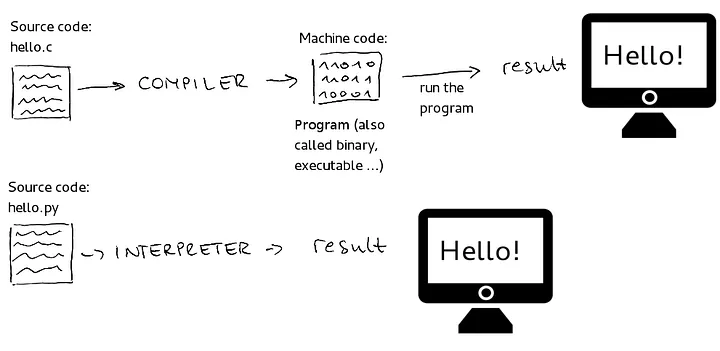
\includegraphics[width=0.8\linewidth]{compiled_vs_interpreted}
%      \end{center}
%    \end{figure}
%  \end{columns}
%\end{frame}
%
%\begin{frame}{Compiled vs Interpreted}
%  \begin{itemize}
%  \item As a result, \texttt{python} is essentially an interactive programming language
%  \item you can program and see the results almost at the same time. 
%  \item \emph{Very nice} when developing a new project since \emph{compilation time} can be quite long (just to give an idea the compilation of our \texttt{C++} financial code takes about one hour). 
%  \item However there are \textbf{drawbacks} in term of performance, the translation to machine language has to be done in real-time resulting in slower execution times.
%  \end{itemize}
%\end{frame}
%
%\begin{frame}{\texttt{python} Language Recap}
%  \begin{itemize}
%    \item Most of you should be already accustomed to \texttt{python}.
%    \item Anyway the first few Chapters of the \href{https://drive.google.com/file/d/1fuVzryJwMCilgynwS7VbWKAmKQBojMQs/view?usp=sharing}{lecture notes} cover in some detail its main features.
%    \item Otherwise you can take a look at one of the thousands \texttt{python} tutorials available on the web.
%    \item Just look at some more advanced aspects here.
%  \end{itemize}
%\end{frame}
%
%\begin{frame}[fragile]{Modules}
%  \begin{itemize}
%  \item Frequently used functions can be written in a \emph{module} and \emph{import} it, instead of copying their definitions into different programs many times.
%  \item In essence modules refer to a file containing \texttt{python} code and used to break down large programs into small manageable and organized files. 
%  \item There are thousands of modules available for \texttt{python} and you can also write your own and distribute it to the community.
%  \item \textbf{The modules we are going to use most are: \texttt{pandas}, \texttt{datetime}, \texttt{matplotlib}, \texttt{scipy}, \texttt{numpy}, \texttt{math}}
%  \item  Lecture notes contain a dedicated Chapter to the first three of them.
%  \end{itemize}
%\end{frame}
%
%\begin{frame}[fragile]{Modules}
%\begin{ipython}
%import math
%help(math)
%\end{ipython}
%\begin{ioutput}
%Help on built-in module math:
%
%NAME
%    math
%
%DESCRIPTION
%    This module provides access to the mathematical functions
%    defined by the C standard.
%
%FUNCTIONS
%    acos(x, /)
%        Return the arc cosine (measured in radians) of x.
%\end{ioutput}
%\begin{ipython}
%dir(math)
%\end{ipython}
%\begin{ioutput}
%['__doc__', '__loader__', '__name__', '__package__', '__spec__', 'acos',
% 'acosh', 'asin', 'asinh', 'atan', 'atan2', 'atanh', ...
%\end{ioutput}    
%\end{frame}
%
%\begin{frame}[fragile]{\texttt{finmarket} Module}
%  \begin{itemize}
%    \item When the function that we want to interpolate is an exponential we can fall back to the previous case by a simple variable transformation. 
%      \begin{equation}
%        \begin{gathered}
%          p = \mathrm{exp}(v \cdot t) \\
%          s = \mathrm{log}(p) = \mathrm{log}(\mathrm{exp}(v \cdot t)) = v \cdot t
%        \end{gathered}
%      \end{equation}
%
%    \item So it is enough to use `numpy.interp` with the lists of $t$ and $\mathrm{log}(p)$ and **to exponentiate back at the end** to get the actual value of $p$.
%    		\begin{ipython}
%    	!pip install --index-url https://test.pypi.org/simple finmarkets
%    \end{ipython}
%    
%  \end{itemize}
%\end{frame}
%
%\begin{frame}[fragile]{\texttt{datetime}}
%	\begin{itemize}
%		\item We will frequently use \texttt{datetime} module, which is dedicated to date and time in \texttt{python}.
%		\item In addition we rely on \texttt{dateutil.relativedelta} to perform operations on dates (dedicated Sections in the notes).
%	\end{itemize}
%	\begin{ipython}
%from datetime import date
%from dateutil.relativedelta import relativedelta
%		
%d = date.today()
%d1 = date(2023, 12, 25)
%print (d, d1, (d1 - d).days)
%print (d1.strftime('%d/%m/%Y'), d1.weekday())
%print (d + relativedelta(days=45))
%print (d + relativedelta(months=45))
%\end{ipython}
%\begin{ioutput}
%2022-09-27 2023-12-25 454
%25/12/2023 0
%2022-11-11
%2026-06-27
%\end{ioutput}
%\end{frame}
%
%\begin{frame}{Payment Dates Generator}
%	\begin{itemize}
%		\item Since we will need to create many lists of dates (e.g. contract payment dates) let's develop an utility that does that for us.
%		\item The function takes as input
%		\begin{itemize}
%			\item \emph{starting date} (the first date of the list);
%			\item \emph{maturity} a string like \texttt{5y} or \texttt{17m} which represents the length of the list;
%			\item \emph{tenor} string like maturity with default value of \texttt{12m}, if the maturity is not a multiple of the tenor the last period will be truncated to the last date.
%		\end{itemize}
%		\item The function returns a list of dates.
%		\end{itemize}		
%\end{frame}
%
%\begin{frame}[fragile]{Payment Dates Generator}
%		\begin{ipython}
%from datetime import date
%from dateutil.relativedelta import relativedelta
%from finmarkets import maturity_from_str
%			
%def generate_dates(start_date, maturity, tenor="1y"):
%	maturity_months = int(round(maturity_from_str(maturity), 0))
%	tenor_months = int(round(maturity_from_str(tenor), 0))
%	dates = []
%	for d in range(0, maturity_months, tenor_months):
%		dates.append(start_date + relativedelta(months=d))
%		dates.append(start_date + relativedelta(months=maturity_months))
%	return dates
%			
%print (generate_dates(date.today(), "25m"))
%\end{ipython}
%\begin{ioutput}
%[datetime.date(2023, 8, 28), datetime.date(2024, 8, 28),
% datetime.date(2025, 8, 28), datetime.date(2025, 9, 28)]
%\end{ioutput}
%\end{frame}
%		
%\begin{frame}{Object Oriented Programming (OOP)}
%	\begin{itemize}
%		\item OOP is a programming model where programs are organized around data, or \textbf{objects}, rather than functions and logic.
%		\item Every object can be thought of as a dataset with unique attributes and behaviour.
%		\item Examples:
%		\begin{itemize}
%			\item a human being that is described by properties like name and birthday;
%			\item the \emph{abstract concepts} of a discount curve with dates and discount factors.
%		\end{itemize}
%	\end{itemize}
%\end{frame}
%
%\begin{frame}{Classes}
%	\begin{itemize}
%		\item Classes are the key ingredient of \emph{Object Oriented Programming}.
%		\item They are implemented in many modern programming language like \texttt{python}, \texttt{Java}, \texttt{C++}\ldots
%		\item In the OOP framework, classes are meant for
%		\begin{itemize}
%			\item creating objects (a particular data structure);
%			\item providing initial values for its state (member variables or attributes);
%			\item implementing their behaviour (member functions or methods).
%		\end{itemize}
%		\item \textbf{A class allows to bundle data and methods that work on that data within one single object.}
%		\item At the very end \emph{classes} are collections of functions that operate on a dataset and \emph{instances} of that class represent individual datasets (or if you prefer a \emph{specialization} of that class).
%	\end{itemize}
%\end{frame}
%
%\begin{frame}{Discount Curve Class}
%	\begin{itemize}
%		\item Import the necessary modules;
%		\item then the \texttt{class} keyword followed by a name is used to start the actual definition;
%		\item define the \emph{constructor} method:
%		\begin{itemize}
%			\item it is always named as \texttt{\_\_init\_\_};
%			\item \textbf{as every other method in a class, takes \texttt{self} as the first argument};
%			\item then any number of parameters as desired by the programmer.
%		\end{itemize}
%		\item \texttt{\_\_init\_\_} allows to specify the initial state of a class by setting its attribute values;
%		\item here, talking about a possible driver, we may want to specify its name and birthday.
%	\end{itemize}
%\end{frame}
%	
%\begin{frame}{Discount Curve Class}
%\begin{itemize}
%	\item \textbf{Attributes} (characteristic data for a curve):
%	\begin{itemize}
%		\item list of pillar dates (corresponding to the given discount factors), $t_0,...,t_{n-1}$;
%		\item list of discount factors, $D(t_0),...,D(t_{n-1})$.
%	\end{itemize}
%	\item \textbf{Methods} ("behaviour" of a discount curve):
%	\begin{itemize}
%		\item one single method returning a discount factor at a given date (if necessary it must interpolate between existing factors);
%		\item the method will use a log-linear interpolation.
%	\end{itemize}
%	\begin{equation*}
%		d(t_i)=\log(D(t_i)) = \log(e^{-r(T-t_i)}) = -r(T-t_i) \;\;\textrm{with }t_i \le t \le t_{i+1}  
%	\end{equation*}
%\end{itemize}
%\end{frame}
%
%\begin{frame}[fragile]{Class Definition}
%\begin{ipython}
%import numpy as np
%	
%from datetime import date
%from scipy.interpolate import interp1d  
%	
%class DiscountCurve:
%  def __init__(self, obs_date, pillar_dates, discount_factors):
%    if obs_date not in pillar_dates:
%	  pillar_dates = [obs_date] + pillar_dates
%      discount_factors = np.insert(np.array(discount_factors), 0, 1)
%    pillar_dates = [d.toordinal() for d in pillar_dates]
%    self.interpolator = interp1d(pillar_Dates, np.log(discount_factors))
%\end{ipython}
%\begin{itemize}
%	\item Variables whose name starts with \texttt{self.} have \emph{class scope}, i.e. are available within each class method.
%	\item Class attributes have to be defined as \texttt{self.variableName = param}
%	\item The \texttt{self.} prefix is used to create and access every attribute or method from within the class itself.
%\end{itemize}
%\end{frame}
%
%\begin{frame}[fragile]{Class Instantiation}
%	\begin{itemize}
%		\item Now that we have the class definition that represents a \emph{generic} discount curve we can specialized it to some \emph{real} curve.
%		\item When \emph{instantiating} a class, \texttt{python} first calls the \texttt{\_\_init\_\_} method and initializes the attributes with the parameter we are passing.
%		\item \textbf{To access class attributes and methods the dot (.) operator has to be used.}
%	\end{itemize}
%\begin{ipython}
%from finmarkets import generate_dates
%			
%pillars = generate_dates(date.today(), "5y")
%dfs = [1, 0.98, 0.97, 0.96, 0.95, 0.94]      
%dc = DiscountCurve(date.today, pillars, dfs)
%print (dc.interpolator.x) # pillars
%print (dc.interpolator.y) # log dfs
%\end{ipython}
%\begin{ioutput}
%Matteo
%\end{ioutput}
%\end{frame}

\begin{frame}[fragile]{First Wrong Implementation}

\begin{ipython}
from datetime import date
from scipy.interpolate import interp1d 

pillars = generate_dates(date.today(), '5y')
dfs = [1, 0.98, 0.97, 0.96, 0.95, 0.94]

def df(d, pillars, dfs):
  interp = interp1d(pillars, dfs)
  return interp(d)
\end{ipython}

\end{frame}		

%\begin{frame}[fragile]{Second Implementation}
%\begin{ipython}	
%pillars = generate_dates(date.today(), "5y")
%dfs = [1, 0.98, 0.97, 0.96, 0.95, 0.94]
%
%def df(d, pillars, dfs):
%  d = d.toordinal()
%  pillars = [d.toordinal() for d in pillars]
%  interp = interp1d(pillars, dfs)
%  return interp(d)
%
%print (df(date(2024, 3, 15), pillars, dfs))
%\end{ipython}
%\begin{ioutput}			
%0.9890710382513661  
%\end{ioutput}
%\end{frame}						

%\begin{frame}[fragile]{Discount Factor Method}
%\begin{ipython}
%import numpy as np
%	
%from datetime import date
%from scipy.interpolate import interp1d  
%	
%class DiscountCurve:
%  def __init__(self, obs_date, pillar_dates, discount_factors):
%    if obs_date not in pillar_dates:
%      pillar_dates = [obs_date] + pillar_dates
%      discount_factors = np.insert(np.array(discount_factors), 0, 1)
%    pillar_dates = [d.toordinal() for d in pillar_dates]
%    self.interpolator = interp1d(pillar_Dates, np.log(discount_factors))
%	
%  def df(self, d):
%    dto = d.toordinal()   
%    if dto < self.interpolator.x[0] or dto > self.interpolator.y[-1]:
%      print (f"Cannot extrapolate discount factors (date: {d}).")
%      return None
%    return np.exp(self.interpolator(dto)
%\end{ipython}
%\end{frame}


\end{document}
